\documentclass{beamer}
\title{Interim Presentation}
\author{Arthur Adriaens}
\date{\today}
\usetheme{Boadilla}
\useoutertheme{infolines}

\begin{document}
\begin{frame}
	\titlepage
\end{frame}
\begin{frame}{Setup}
  \begin{itemize}
    \item principle
    \item The need for RNO-G
    \item RNO-G
    \item Ice Models
    \item Iterative Ray Tracer
    \item Hybrid Ray Tracer
  \end{itemize}
\end{frame}
\begin{frame}{Principle}
  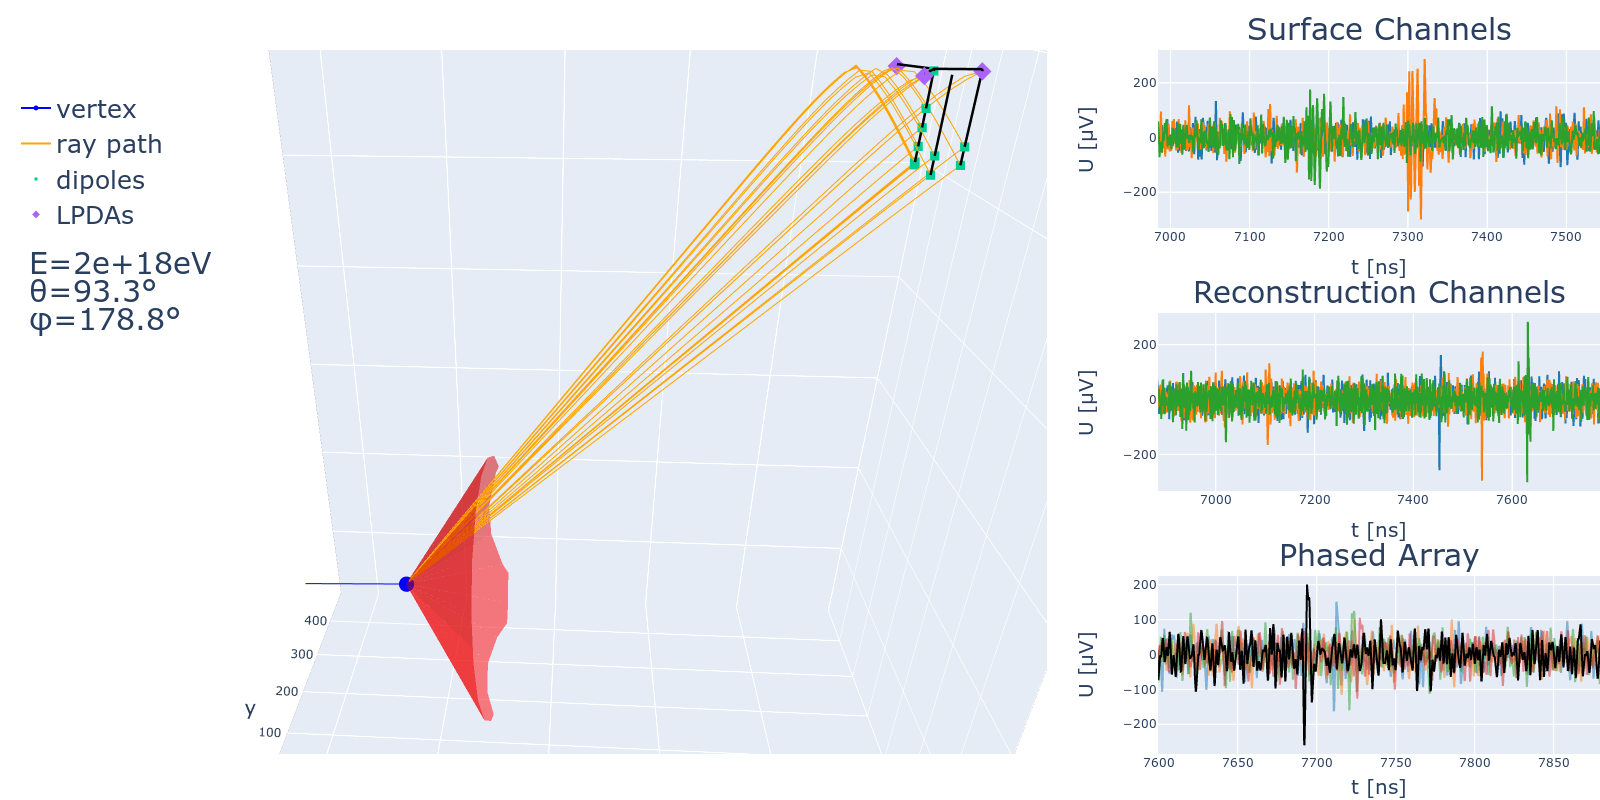
\includegraphics[width=\textwidth]{figures/mechanism.png}
\end{frame}
\begin{frame}{The need for RNO-G}
  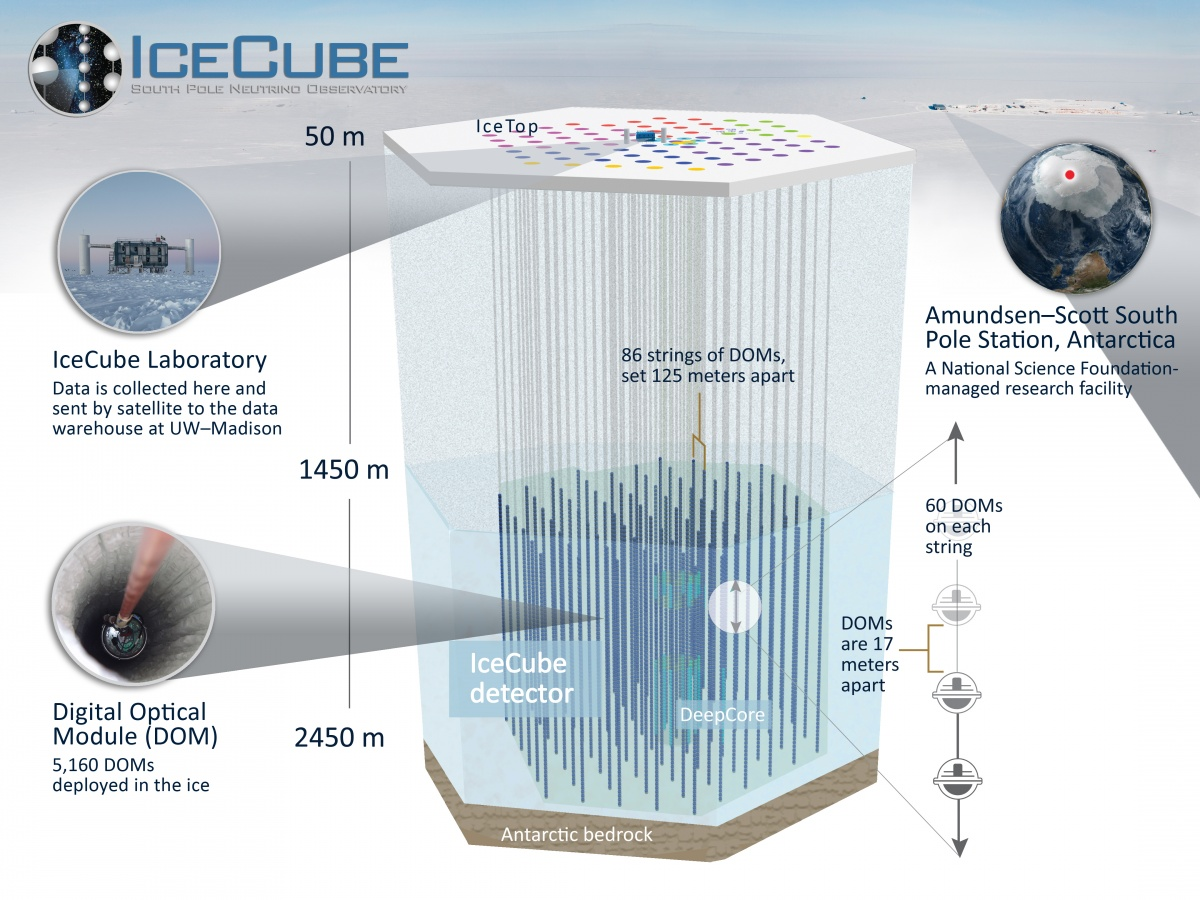
\includegraphics[height=0.9\textheight]{figures/icecube.jpg}
\end{frame}
\begin{frame}{The need for RNO-G}
  \centering
  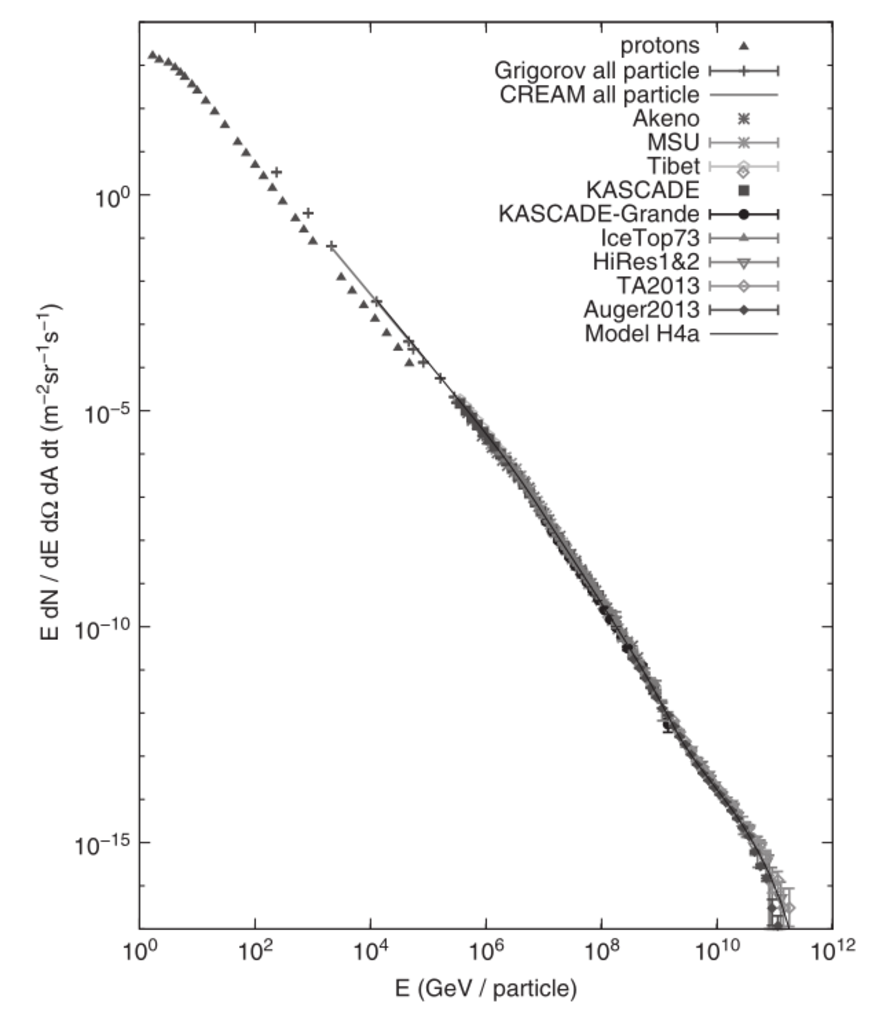
\includegraphics[height=0.9\textheight]{figures/cosmic_ray_flux.pdf}
\end{frame}
\begin{frame}{The need for RNO-G}
\begin{itemize}
	\item IceCube finds no events for energies $> 3PeV$ (\it{IceCube study of down-going neutrinos for the spectral cutoff determination by Palczewski and Tomasz})
\end{itemize}
\end{frame}
\begin{frame}{RNO-G}
  Problem: visible light doesn't travel far in ice\\
  $\rightarrow$ Solution: radio waves
\end{frame}
\begin{frame}{RNO-G}
  \centering
  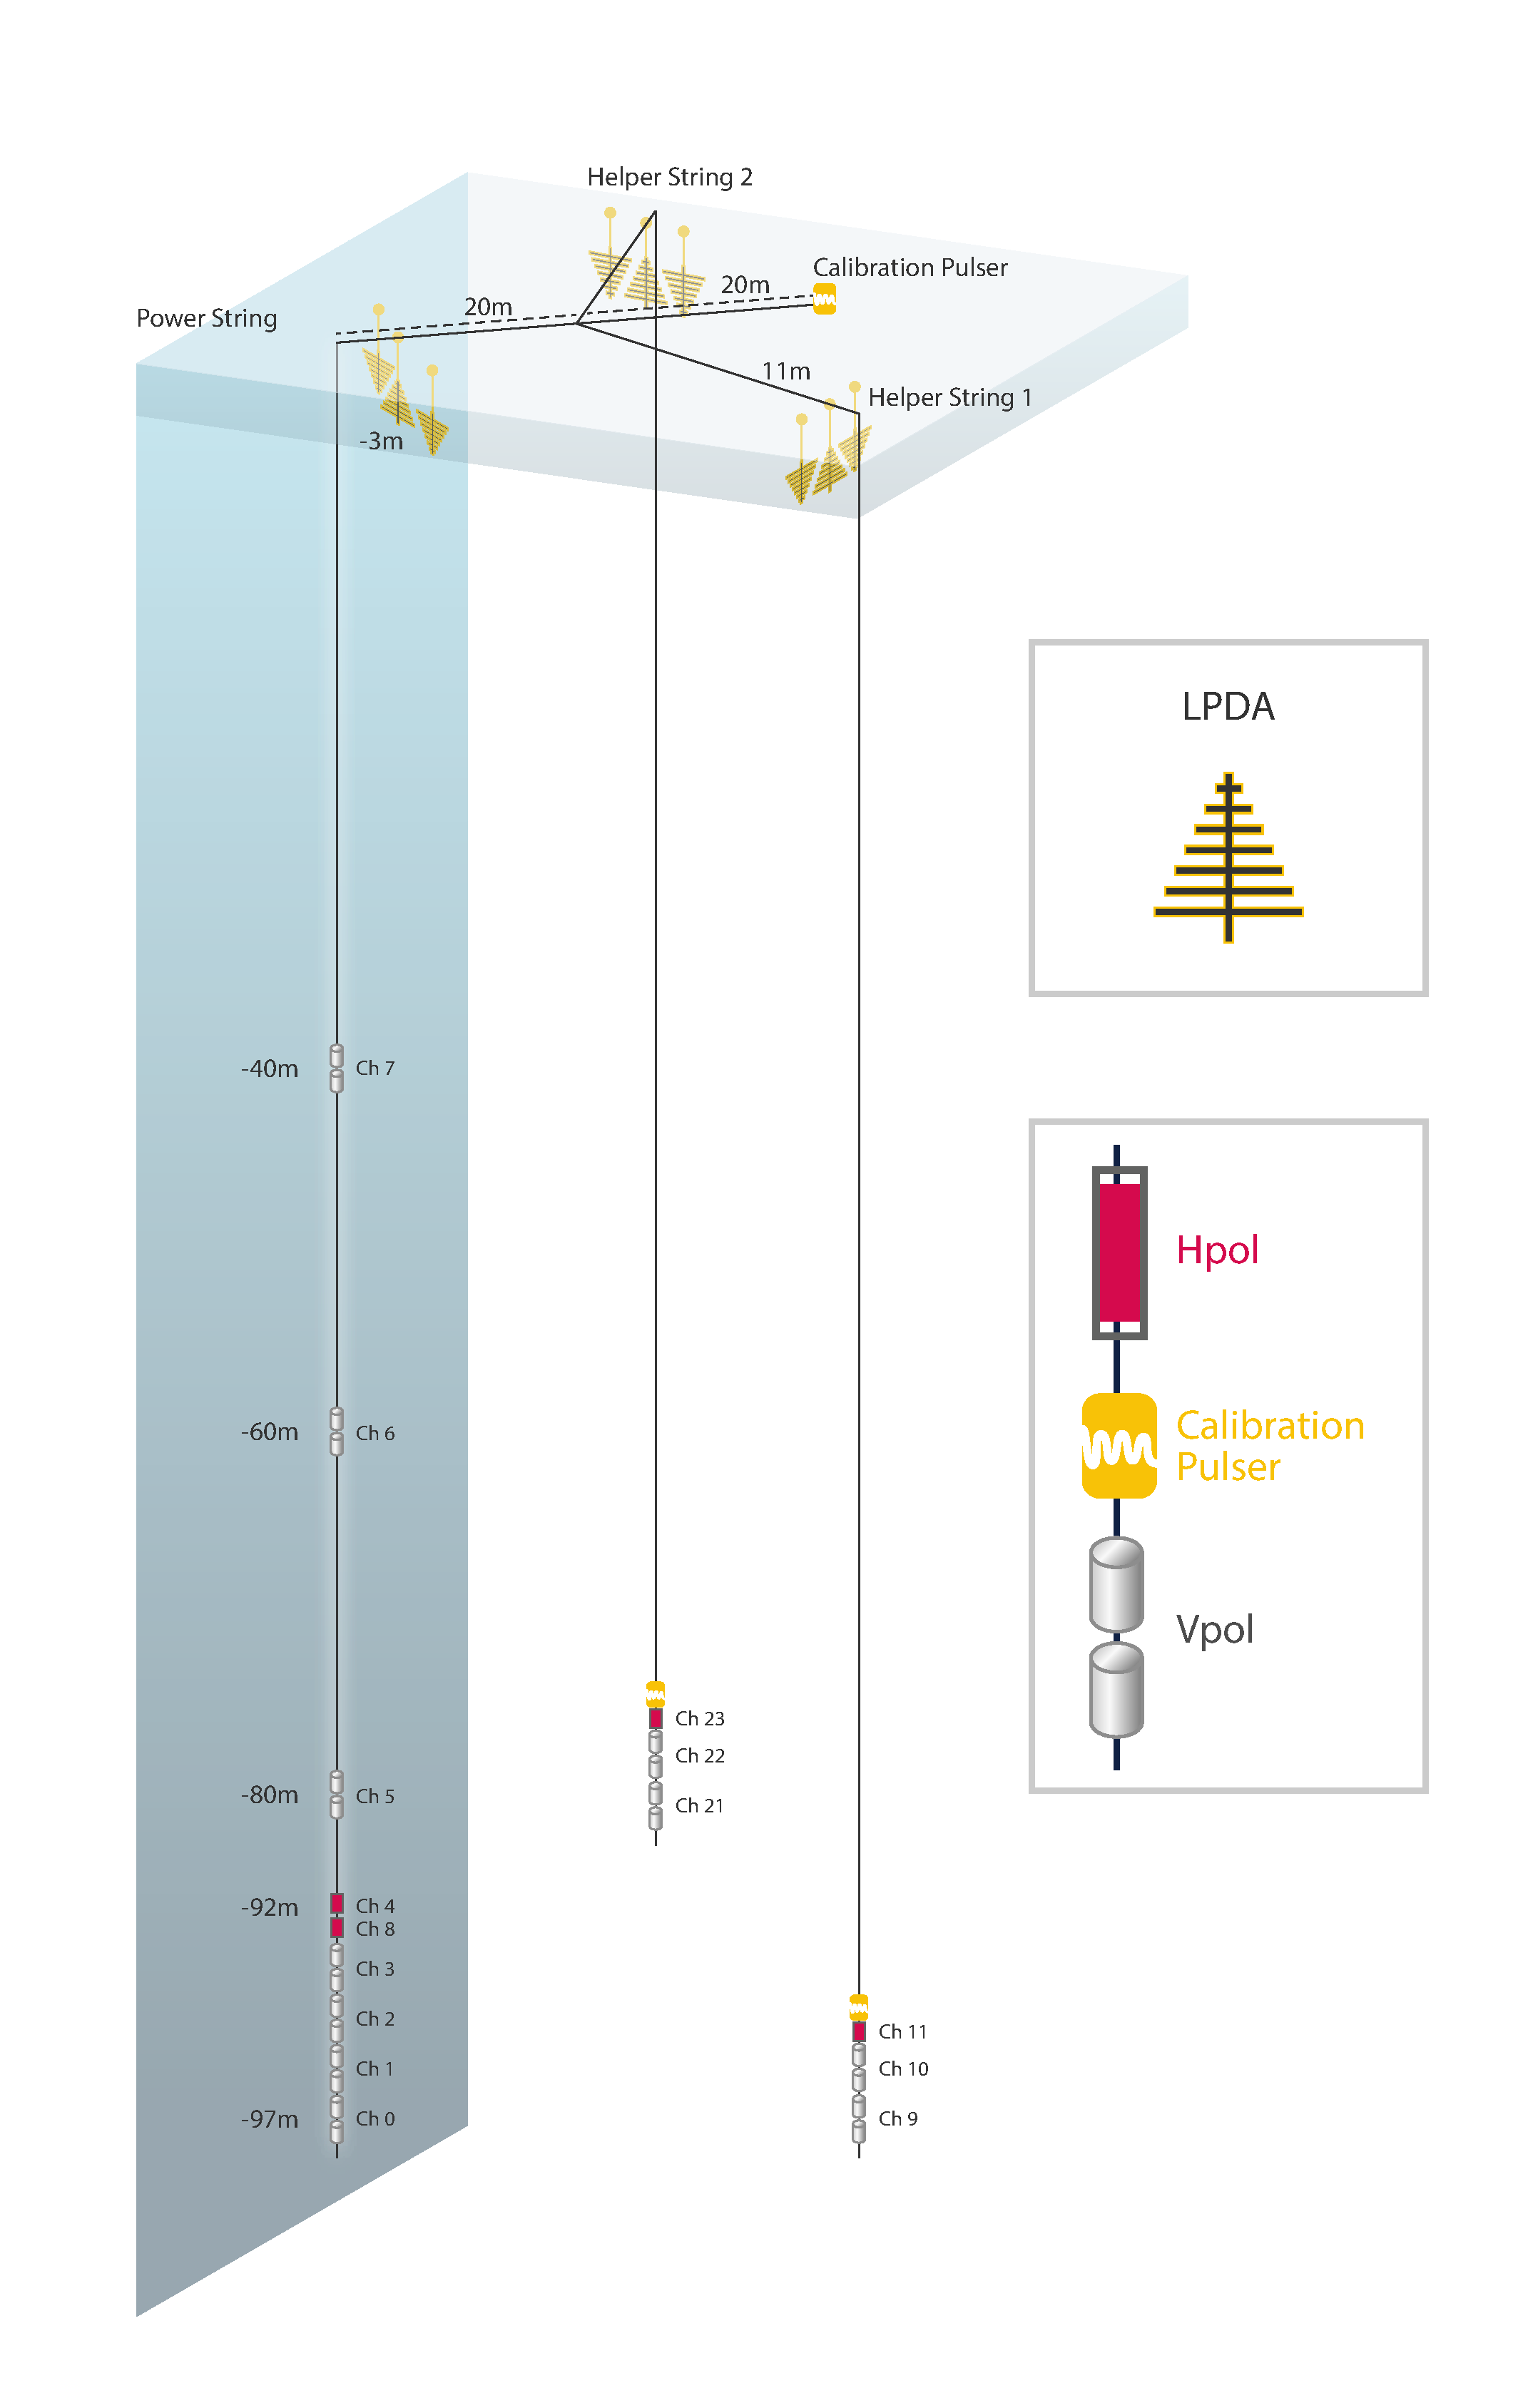
\includegraphics[height=0.9\textheight]{figures/detector.pdf}
\end{frame}
\begin{frame}{RNO-G}
  \centering
  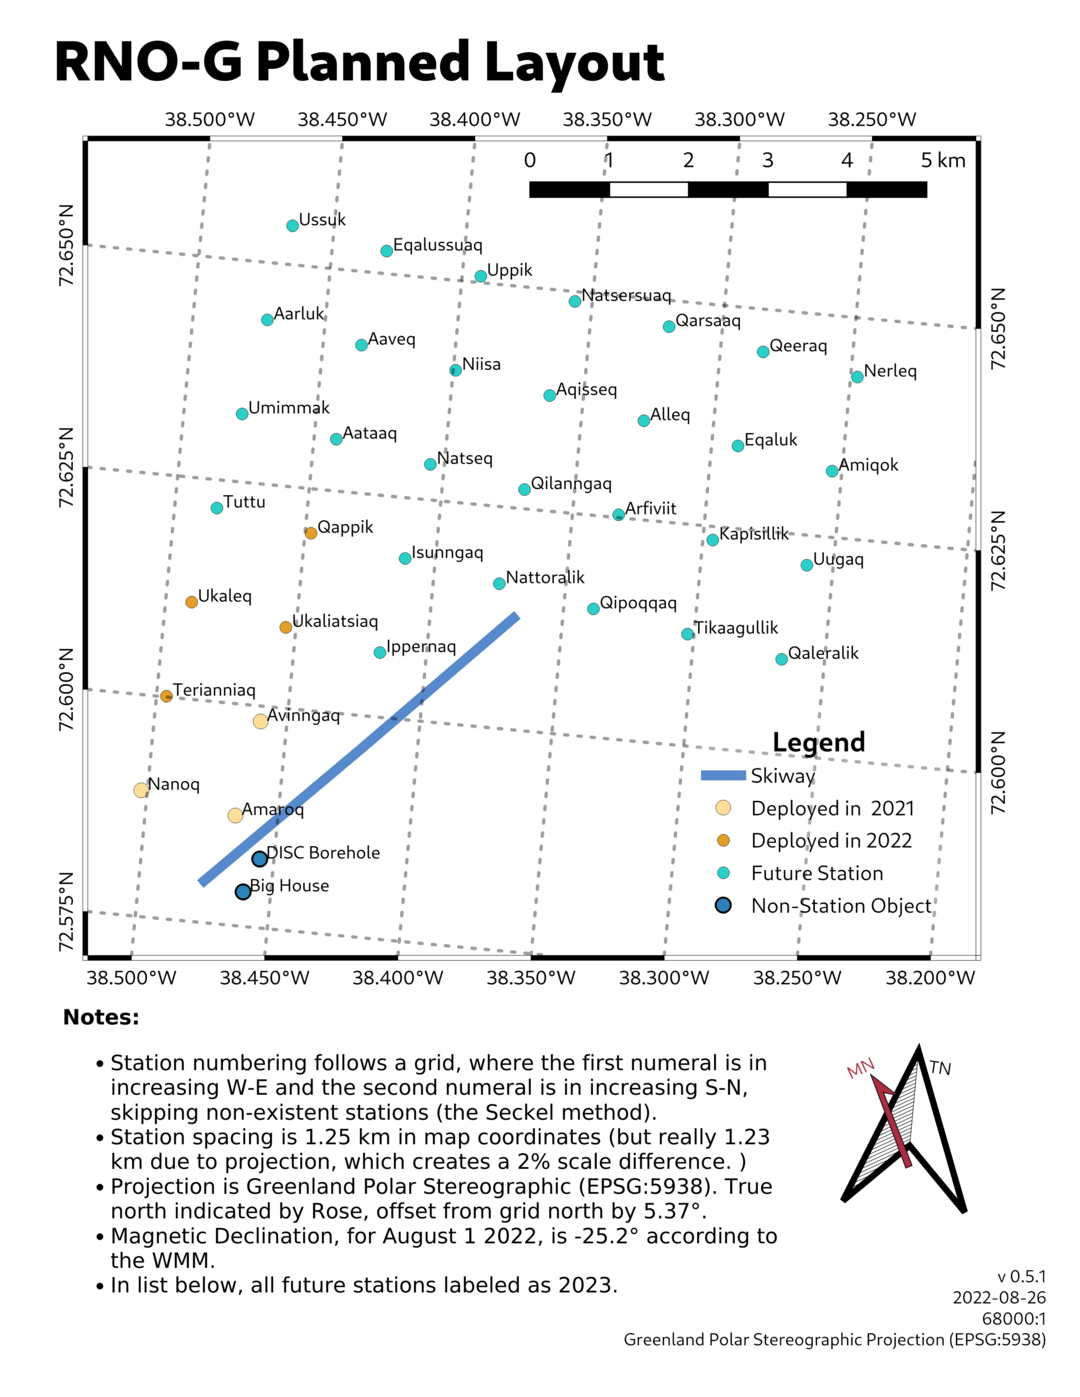
\includegraphics[height=\textheight]{figures/station-map.png}
\end{frame}
\begin{frame}
  \centering
  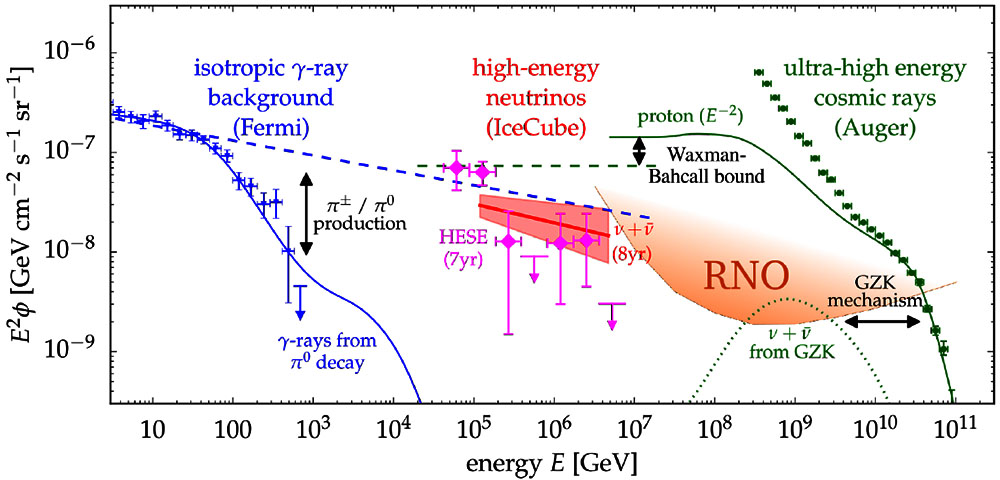
\includegraphics[width=\textwidth]{figures/range.jpg}
\end{frame}
\begin{frame}{RNO-G}
	"A Pathfinder for IceCube-Gen2 Radio"
\end{frame}
\begin{frame}{Ice Models}
  \centering
  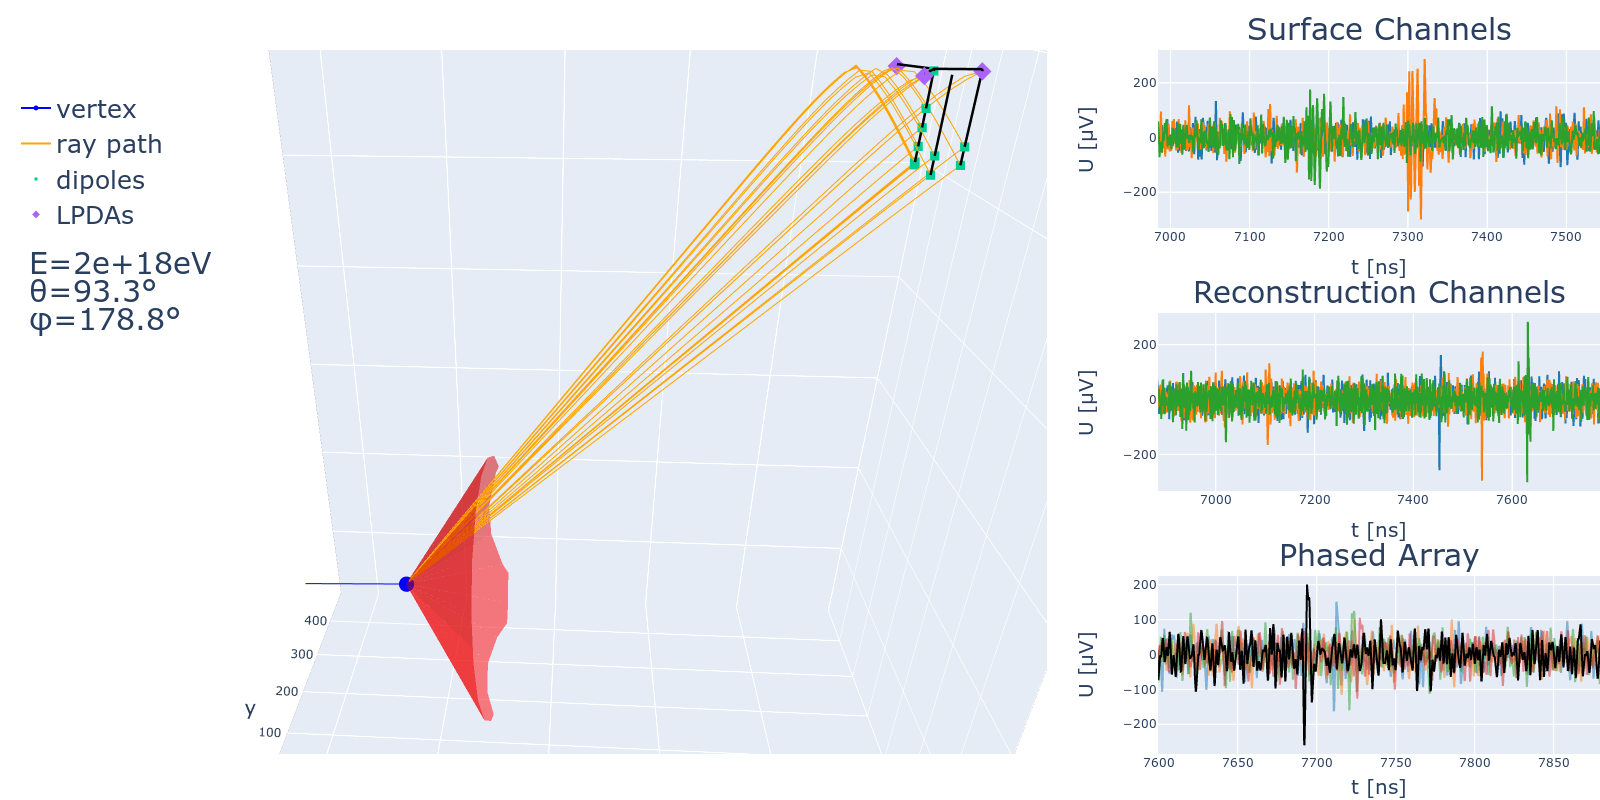
\includegraphics[width=\textwidth]{figures/mechanism.png}
\end{frame}
\begin{frame}{Ice Models}
Eikonal:
  \begin{equation}
    \mathbf{\nabla} n \approx n(\mathbf{r})\frac{d^2\mathbf{r}}{ds^2}
  \end{equation}
\begin{figure}
\centering
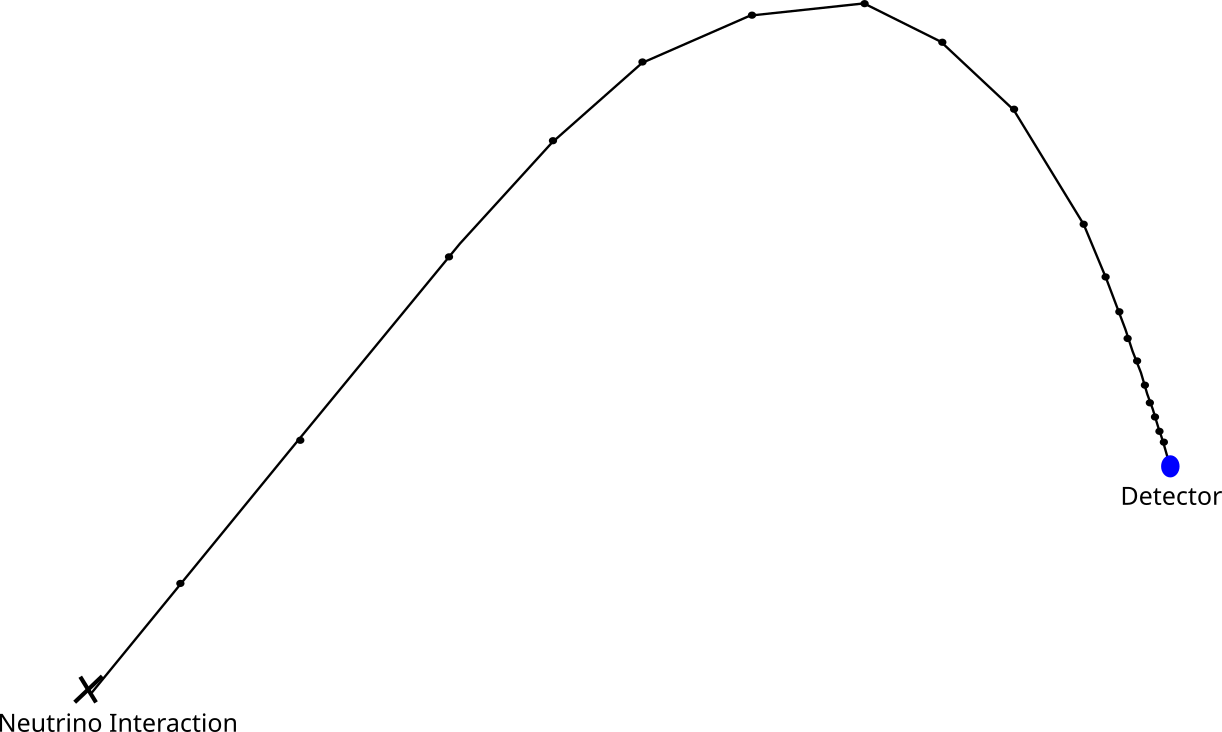
\includegraphics[width=0.5\textwidth]{figures/ExplanationRadiopropa.png}
\end{figure}
Exponential model:
  \begin{equation}
    n(z) = n_0 - \Delta n \ e^{-z/z_0}
  \end{equation}
\end{frame}
\begin{frame}{Ice Models}
  \centering
  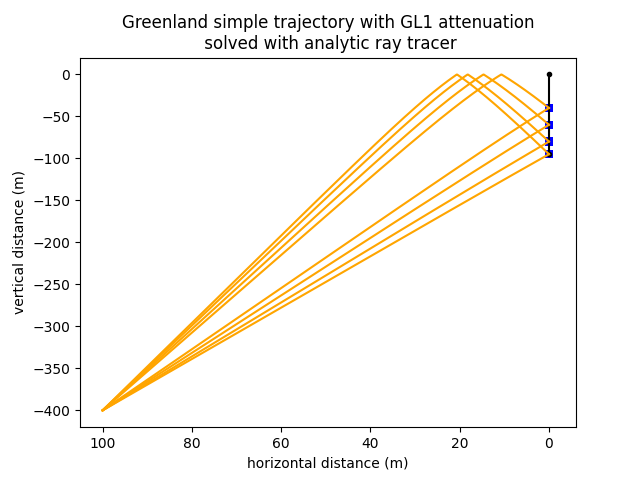
\includegraphics[width=\textwidth]{figures/detector-illustration.png}
\end{frame}
\begin{frame}{Iterative Ray tracer}
  \centering
  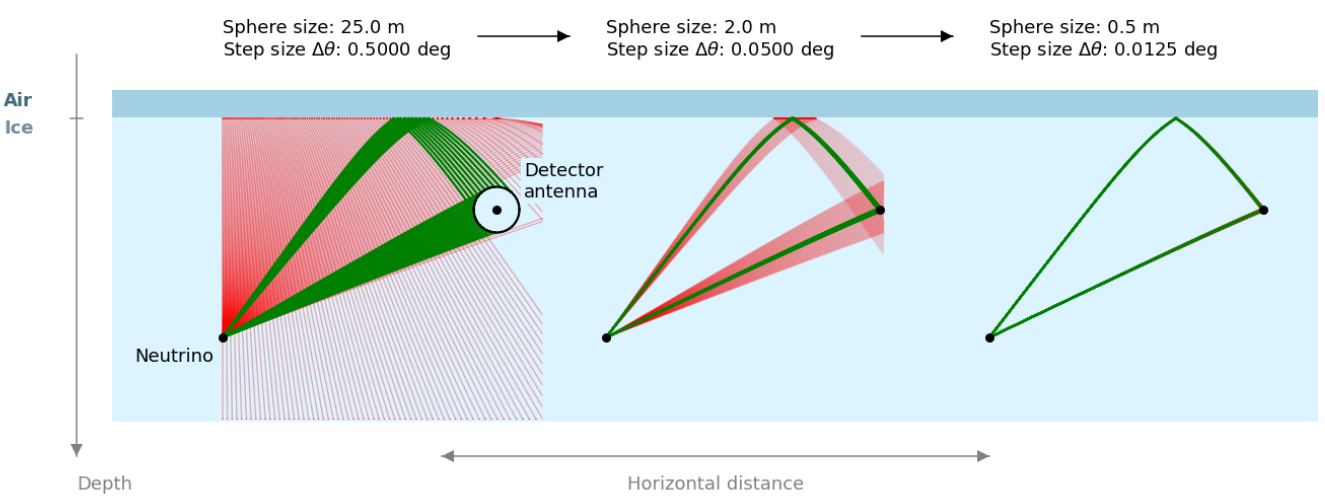
\includegraphics[width=\textwidth]{figures/iterative_explanation.png}
\end{frame}
\begin{frame}{Hybrid Ray tracer}
	What we want?: Scipy
\end{frame}
\begin{frame}{Hybrid Ray tracer}
  \centering
  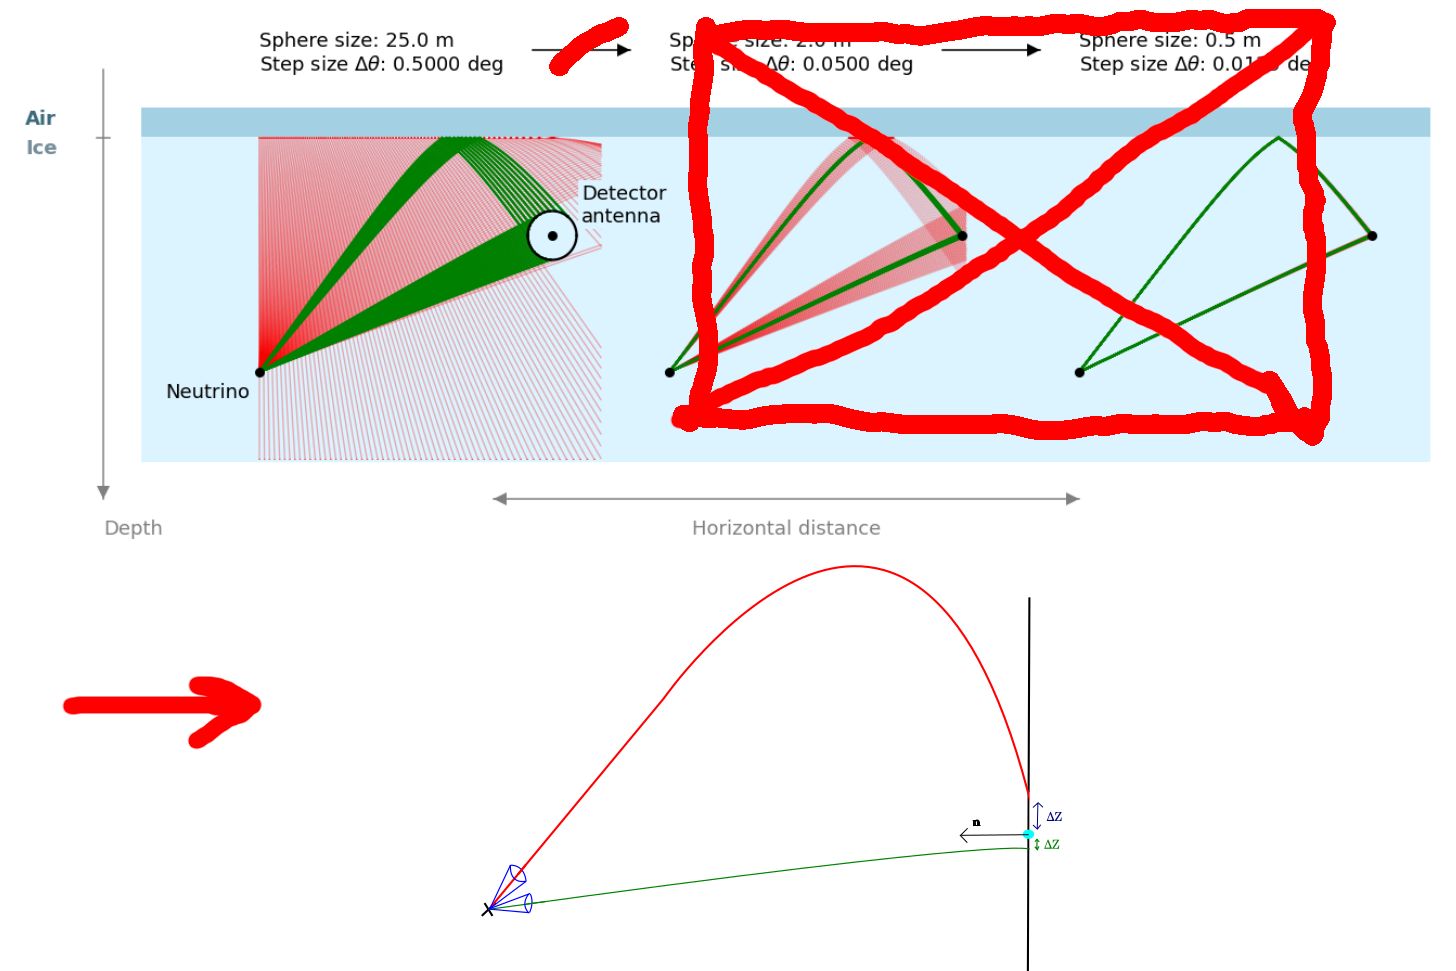
\includegraphics[width=\textwidth]{figures/FullHybridIllu.png}
\end{frame}
\begin{frame}{Hybrid Ray tracer: Optimization}
  \centering
  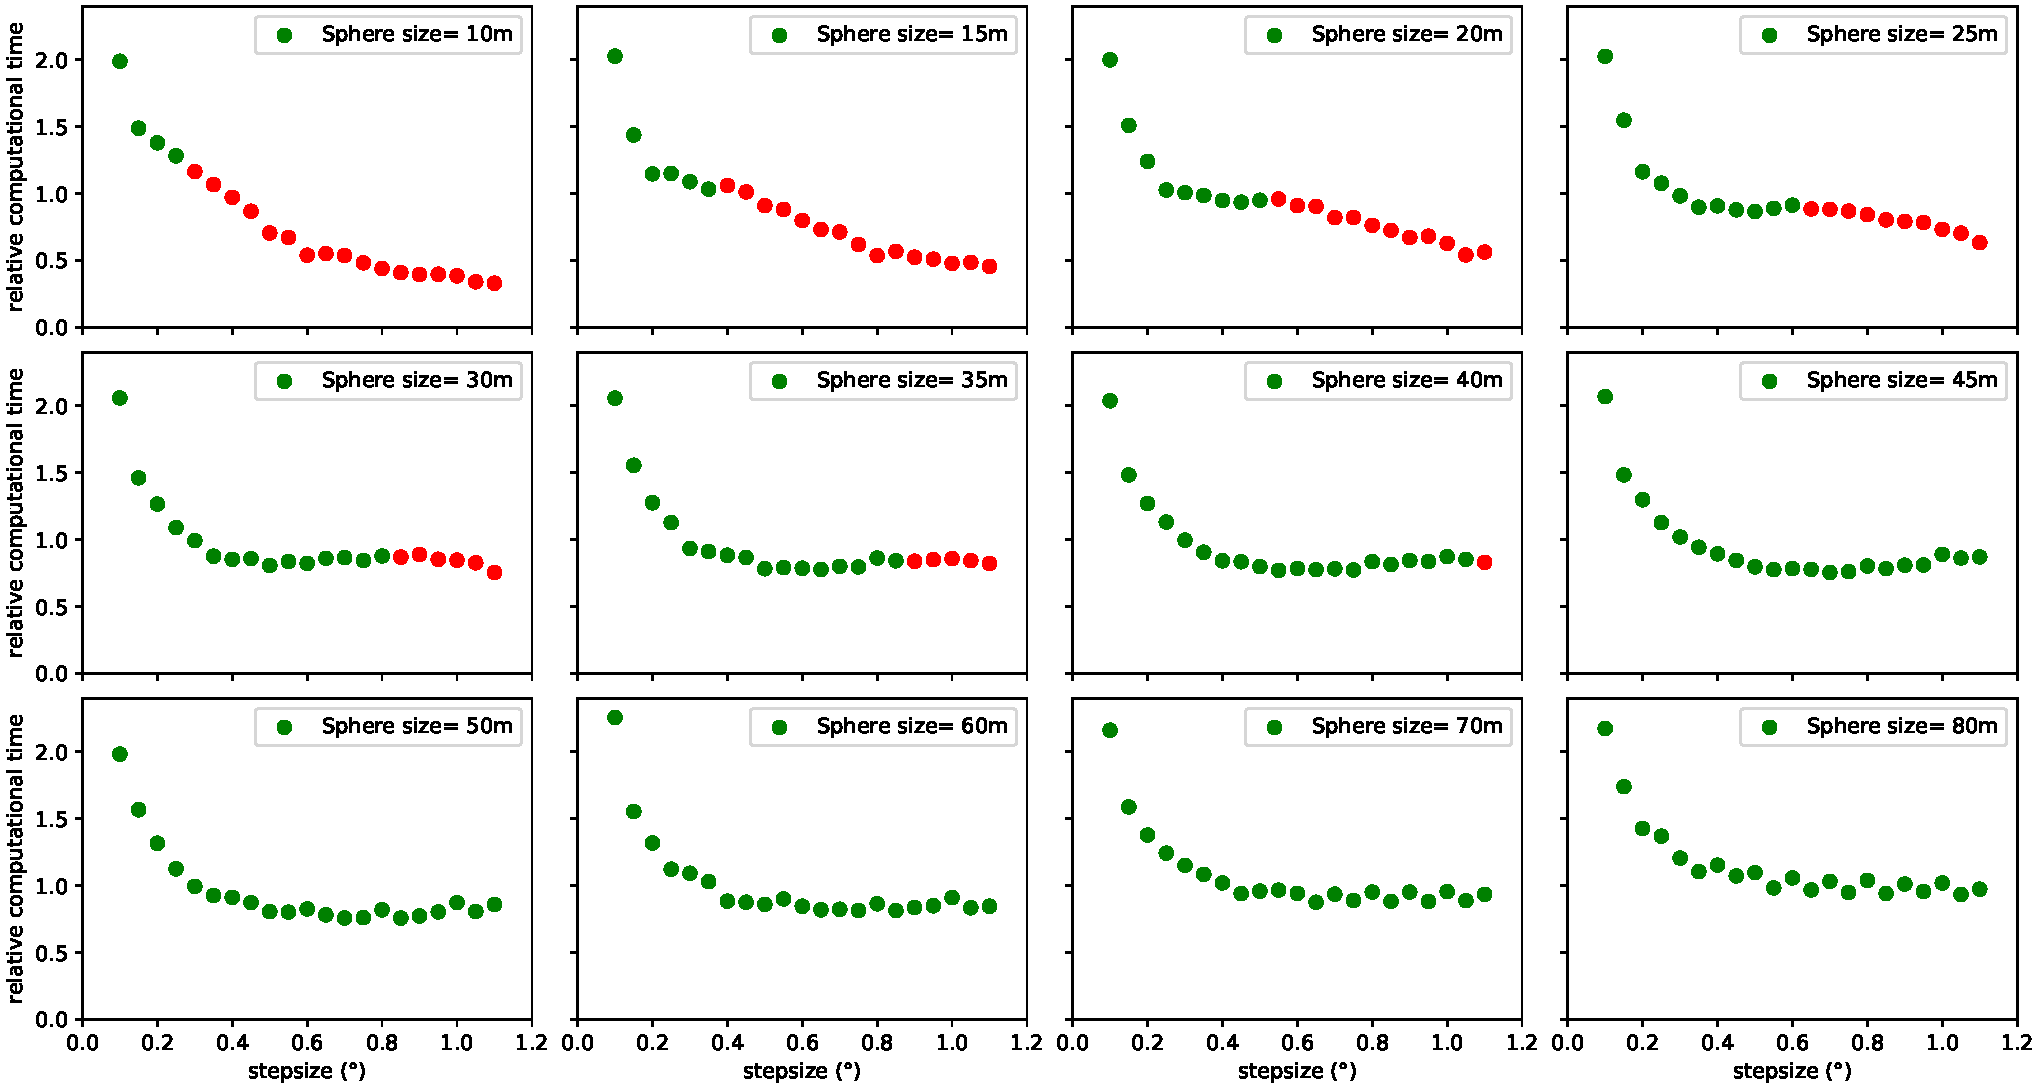
\includegraphics[width=\textwidth]{figures/subplotallsphereandstep.pdf}
\end{frame}
\begin{frame}{Hybrid Ray tracer: Optimization}
	\begin{minipage}{0.49\textwidth}
	\begin{figure}
		\centering
		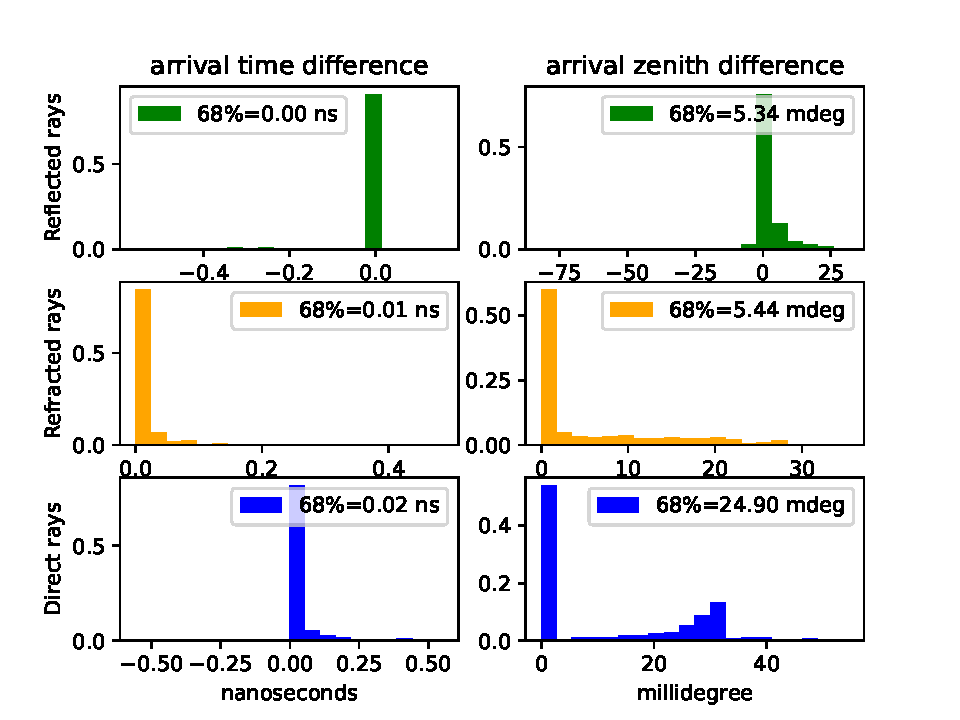
\includegraphics[width=\textwidth]{figures/hybrid_comparison_N_500.pdf}
		\caption{Hybrid}
	\end{figure}
	\end{minipage}
	\begin{minipage}{0.49\textwidth}
	\begin{figure}
		\centering
		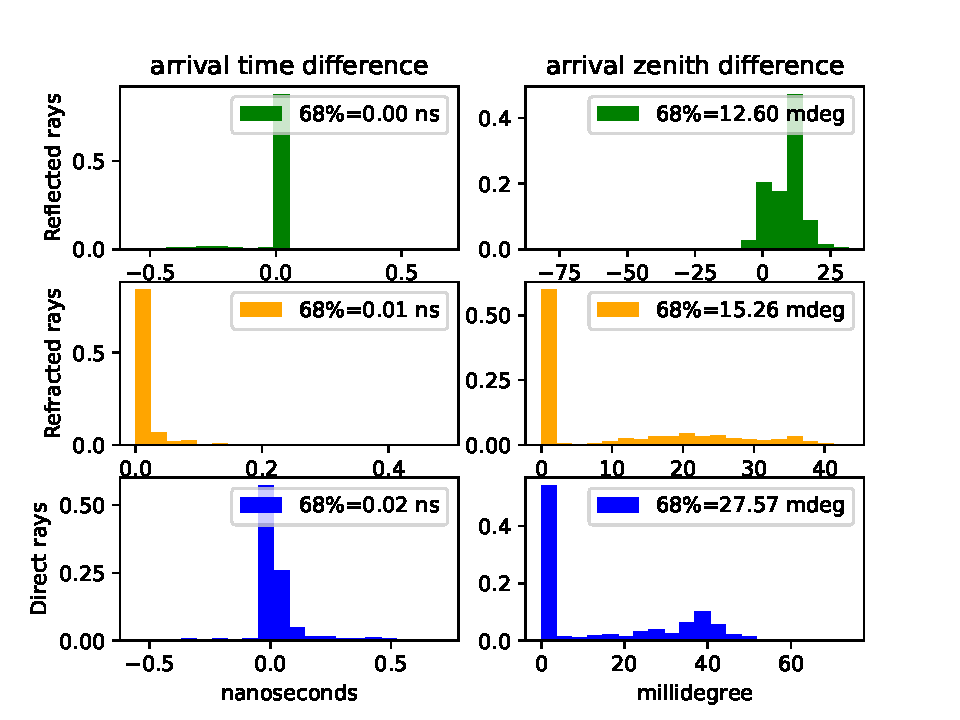
\includegraphics[width=\textwidth]{figures/iterative_comparison_N_500.pdf}
		\caption{Iterative}
	\end{figure}
	\end{minipage}
i.e more accurate whilst being $\approx$ 30\% faster (30\% more computations per second) than the iterative ray tracer
\end{frame}
\end{document}
